\usetikzlibrary{arrows.meta}
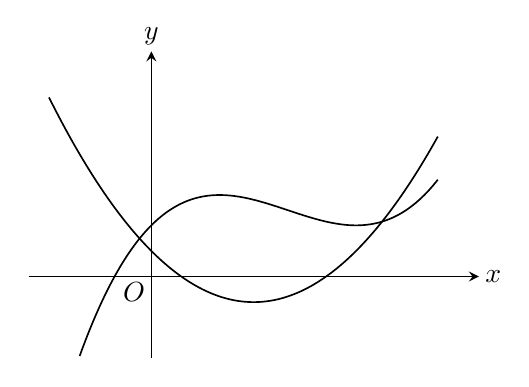
\begin{tikzpicture}[x=1.3cm,y=1.3cm,line width=.6pt,>=stealth,font=\normalsize]
\draw[->] (-1.2,0)--(3.2,0) node[right,inner sep=0pt,xshift=2pt] {$x$};
\draw[->] (0,-0.8)--(0,2.2) node[above,inner sep=0pt,yshift=2pt] {$y$};
\node[below left,inner sep=0pt,xshift=-2pt,yshift=-2pt] at (0,0) {$O$};
\draw[domain=-1.0:2.8,samples=120] plot (\x,{0.5*\x*\x-\x+0.25});
\draw[domain=-0.7:2.8,samples=160] plot (\x,{0.25*\x*\x*\x-\x*\x+\x+0.5});
\end{tikzpicture}
